\documentclass[11pt]{article}
\usepackage[margin=1in]{geometry}
\usepackage{amsmath,amssymb,amsthm}
\usepackage{tikz}
\usepackage{mathtools}

\newcommand{\encode}{\operatorname{encode}}

\title{Meandric systems from Thompson's group elements}
\author{}
\date{}

\begin{document}
\maketitle

\section{Binary trees and noncrossing pairings}

Every element of Thompson's group $F$ is represented by a pair of finite rooted binary trees $(T_-, T_+)$ with the same number of leaves $n+1$, where both trees have $n$ internal nodes.  A binary tree with $n$ internal nodes can be encoded as a noncrossing perfect pairing on $\{1, 2, \ldots, 2n\}$ via the following recursive rule.  If $v$ is an internal node with left subtree $L$ and right subtree $R$, define
\[
  \encode(v) \;=\; U \cdot \encode(L) \cdot D \cdot \encode(R),
\]
where a leaf encodes as the empty word.  The resulting word is a Dyck path of semilength $n$.  Matching each $U$ step with the $D$ step that returns the path to the same level produces a noncrossing perfect pairing on $\{1, \ldots, 2n\}$.

Given a tree pair $(T_-, T_+)$, we place the noncrossing pairing of $T_-$ as arcs \emph{above} a horizontal row of $2n$ points, and the pairing of $T_+$ as arcs \emph{below}.  Together they form what we call a \textbf{meandric system}: a collection of closed curves obtained by alternately traversing top and bottom arcs.

The number of connected components of the meandric system equals the number of orbits of the permutation $\sigma_- \circ \sigma_+^{-1}$, where $\sigma_\pm$ are the fixed-point-free involutions corresponding to the two pairings.  The faces of the meandric system (connected regions of the complement) correspond to the leaves of the trees, i.e., to the linear pieces of the PL homeomorphism.

\subsection*{Why the encoding is asymmetric}

A natural first reaction to the encoding rule
\[
  \encode(v) \;=\; U \cdot \encode(L) \cdot D \cdot \encode(R)
\]
is that it treats left and right subtrees very differently.  Indeed it does, and this is not an accident --- it is forced by the Dyck path constraint.  To see why, note that the $U$ and $D$ contributed by the node $v$ itself form a matched pair of parentheses.  The left subtree $L$ is encoded \emph{inside} this pair of parentheses (between $U$ and $D$), while the right subtree $R$ is encoded \emph{after} the closing parenthesis $D$.  In bracket notation:
\[
  \underbrace{(\;\overbrace{\encode(L)}^{\text{inside}}\;)}_{\text{from } v}\;\;\underbrace{\encode(R)}_{\text{after}}.
\]
As a consequence, mirror-image trees produce genuinely different Dyck paths.  For instance, in the tree pair for $x_0$:

\begin{center}
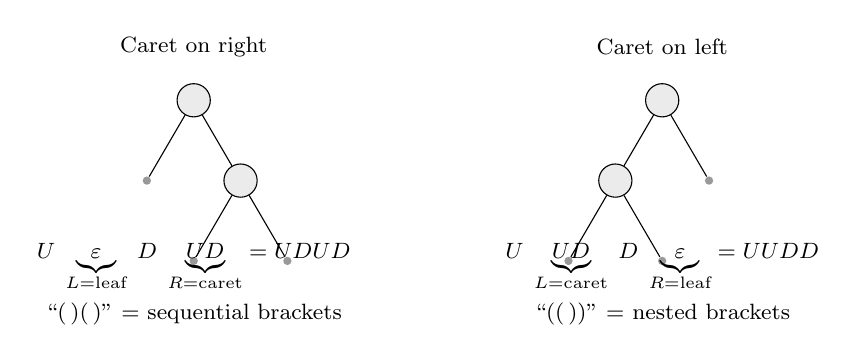
\begin{tikzpicture}[
  inode/.style={circle, draw, fill=black!8, inner sep=0pt, minimum size=12pt},
  leaf/.style={circle, fill=black!40, inner sep=0pt, minimum size=3pt},
  level distance=12mm, sibling distance=14mm,
  edge from parent/.style={draw, thin},
  scale=0.85
]
% Left: caret on right
\node at (-3.5, 1.2) {\footnotesize Caret on right};
\node[inode] (r1) at (-3.5, 0.4) {}
  child { node[leaf] {} }
  child { node[inode] {}
    child { node[leaf] {} }
    child { node[leaf] {} }
  };
\node at (-3.5, -2.1) {\footnotesize $U\;\underbrace{\varepsilon}_{L=\text{leaf}}\;D\;\underbrace{UD}_{R=\text{caret}} = UDUD$};
\node at (-3.5, -2.8) {\footnotesize ``$(\,)(\,)$'' $=$ sequential brackets};

% Right: caret on left
\node at (3.5, 1.2) {\footnotesize Caret on left};
\node[inode] (r2) at (3.5, 0.4) {}
  child { node[inode] {}
    child { node[leaf] {} }
    child { node[leaf] {} }
  }
  child { node[leaf] {} };
\node at (3.5, -2.1) {\footnotesize $U\;\underbrace{UD}_{L=\text{caret}}\;D\;\underbrace{\varepsilon}_{R=\text{leaf}} = UUDD$};
\node at (3.5, -2.8) {\footnotesize ``$((\,))$'' $=$ nested brackets};
\end{tikzpicture}
\end{center}

\noindent When the caret is on the \emph{right}, the left subtree is a leaf (contributing~$\varepsilon$ inside the brackets), so the brackets from the root close immediately, and the caret's own brackets follow \emph{after}: $(\,)(\,) = UDUD$.  When the caret is on the \emph{left}, its encoding is inserted \emph{inside} the root's brackets, producing a nested structure: $((\,)) = UUDD$.

In general:
\begin{itemize}
\item A right-leaning tree (a chain of right children) produces the path $UDUDUD\cdots$, a sequence of independent bumps --- each internal node opens and closes its own brackets with nothing inside.
\item A left-leaning tree (a chain of left children) produces $UU\cdots DD\cdots$, a single tall mountain --- each node's brackets are nested inside its parent's.
\end{itemize}

One might ask: could we choose a symmetric rule, say $\encode(v) = U \cdot \encode(L) \cdot \encode(R) \cdot D$, where \emph{both} subtrees sit inside the brackets?  The resulting word would still have $n$ copies of~$U$ and $n$ copies of~$D$, but it would not in general be a Dyck path: the path could dip below level~$0$ between $\encode(L)$ and $\encode(R)$.  Our asymmetric rule is the unique way to map binary trees bijectively to Dyck paths so that each internal node corresponds to exactly one matched pair of parentheses.

\section{The generator $x_0$}

The generator $x_0 \in F$ is the PL homeomorphism
\[
  x_0(t) = \begin{cases}
    t/2, & t \in [0, 1/2], \\
    t - 1/4, & t \in [1/2, 3/4], \\
    2t - 1, & t \in [3/4, 1].
  \end{cases}
\]

\noindent\textbf{Tree pair.}  The domain tree $T_-$ has a caret on the right child of the root (encoding the subdivision $\{0, \tfrac{1}{2}, \tfrac{3}{4}, 1\}$), while the range tree $T_+$ has a caret on the left child (encoding $\{0, \tfrac{1}{4}, \tfrac{1}{2}, 1\}$).  Both have $n = 2$ internal nodes and $3$ leaves.

\medskip
\begin{center}
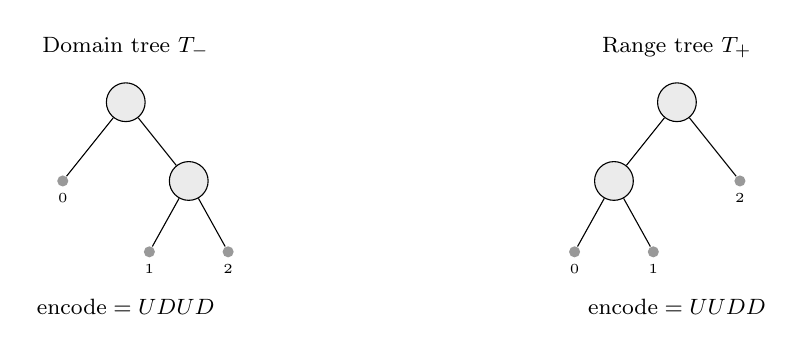
\begin{tikzpicture}[
  inode/.style={circle, draw, fill=black!8, inner sep=0pt, minimum size=14pt, font=\footnotesize},
  leaf/.style={circle, fill=black!40, inner sep=0pt, minimum size=4pt},
  scale=1
]
% Domain tree
\node at (-3.5, 1.7) {\footnotesize Domain tree $T_-$};
\node[inode] (a) at (-3.5, 1) {};
\node[leaf]  (l0) at (-4.3, 0) {};
\node[inode] (b) at (-2.7, 0) {};
\node[leaf]  (l1) at (-3.2, -0.9) {};
\node[leaf]  (l2) at (-2.2, -0.9) {};
\draw (a) -- (l0);
\draw (a) -- (b);
\draw (b) -- (l1);
\draw (b) -- (l2);
\node[font=\tiny, below=1pt] at (l0) {$0$};
\node[font=\tiny, below=1pt] at (l1) {$1$};
\node[font=\tiny, below=1pt] at (l2) {$2$};

% Range tree
\node at (3.5, 1.7) {\footnotesize Range tree $T_+$};
\node[inode] (c) at (3.5, 1) {};
\node[inode] (d) at (2.7, 0) {};
\node[leaf]  (l5) at (4.3, 0) {};
\node[leaf]  (l3) at (2.2, -0.9) {};
\node[leaf]  (l4) at (3.2, -0.9) {};
\draw (c) -- (d);
\draw (c) -- (l5);
\draw (d) -- (l3);
\draw (d) -- (l4);
\node[font=\tiny, below=1pt] at (l3) {$0$};
\node[font=\tiny, below=1pt] at (l4) {$1$};
\node[font=\tiny, below=1pt] at (l5) {$2$};

% Encodings
\node at (-3.5, -1.6) {\footnotesize $\encode = UDUD$};
\node at (3.5, -1.6) {\footnotesize $\encode = UUDD$};
\end{tikzpicture}
\end{center}

\noindent\textbf{Noncrossing pairings.}
\begin{align*}
  T_- &: UDUD \;\longrightarrow\; \{1,2\},\;\{3,4\}, \\
  T_+ &: UUDD \;\longrightarrow\; \{1,4\},\;\{2,3\}.
\end{align*}

\noindent\textbf{Meandric system.}  Placing the domain pairing on top and the range pairing on the bottom:

\begin{center}
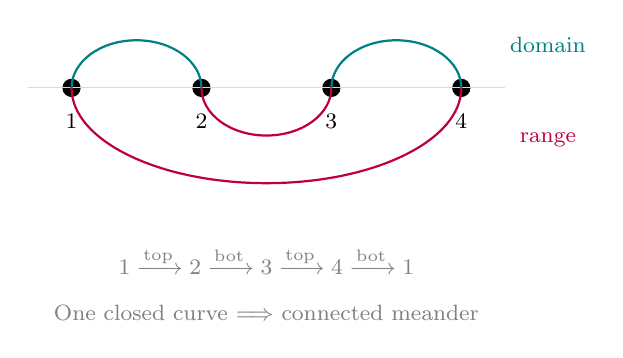
\begin{tikzpicture}[scale=1.1]
  % Points
  \foreach \i/\x in {1/0, 2/1.5, 3/3, 4/4.5} {
    \fill (\x, 0) circle (3pt);
    \node[below=6pt, font=\footnotesize] at (\x, 0) {$\i$};
  }

  % Horizontal line
  \draw[gray!30] (-0.5, 0) -- (5, 0);

  % Top arcs (domain): {1,2}, {3,4}
  \draw[teal, thick] (0,0) arc[start angle=180, end angle=0, x radius=0.75, y radius=0.55];
  \draw[teal, thick] (3,0) arc[start angle=180, end angle=0, x radius=0.75, y radius=0.55];
  \node[teal, font=\footnotesize] at (5.5, 0.5) {domain};

  % Bottom arcs (range): {1,4}, {2,3}
  \draw[purple, thick] (0,0) arc[start angle=180, end angle=360, x radius=2.25, y radius=1.1];
  \draw[purple, thick] (1.5,0) arc[start angle=180, end angle=360, x radius=0.75, y radius=0.55];
  \node[purple, font=\footnotesize] at (5.5, -0.6) {range};

  % Trace annotation
  \node[font=\footnotesize, gray] at (2.25, -2) {$1 \xrightarrow{\text{top}} 2 \xrightarrow{\text{bot}} 3 \xrightarrow{\text{top}} 4 \xrightarrow{\text{bot}} 1$};
  \node[font=\footnotesize, gray] at (2.25, -2.6) {One closed curve $\Longrightarrow$ connected meander};
\end{tikzpicture}
\end{center}

The meandric system for $x_0$ consists of a single closed curve passing through all $4$ points.  Its complement has $3$ faces, corresponding to the $3$ strands (linear pieces) of $x_0$.

\section{The generator $x_1$}

The generator $x_1 \in F$ is the identity on $[0, 1/2]$ and acts like a rescaled copy of $x_0$ on $[1/2, 1]$:
\[
  x_1(t) = \begin{cases}
    t, & t \in [0, 1/2], \\
    t/2 + 1/4, & t \in [1/2, 3/4], \\
    t - 1/8, & t \in [3/4, 7/8], \\
    2t - 1, & t \in [7/8, 1].
  \end{cases}
\]

\noindent\textbf{Tree pair.}  Both trees have $n = 3$ internal nodes and $4$ leaves.

\medskip
\begin{center}
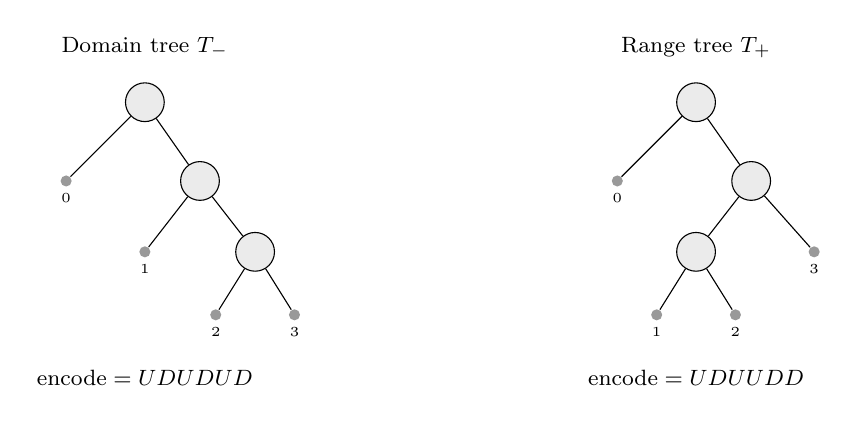
\begin{tikzpicture}[
  inode/.style={circle, draw, fill=black!8, inner sep=0pt, minimum size=14pt, font=\footnotesize},
  leaf/.style={circle, fill=black!40, inner sep=0pt, minimum size=4pt},
  scale=1
]
% Domain tree: right chain
\node at (-3.5, 2.2) {\footnotesize Domain tree $T_-$};
\node[inode] (a) at (-3.5, 1.5) {};
\node[leaf]  (l0) at (-4.5, 0.5) {};
\node[inode] (b) at (-2.8, 0.5) {};
\node[leaf]  (l1) at (-3.5, -0.4) {};
\node[inode] (c) at (-2.1, -0.4) {};
\node[leaf]  (l2) at (-2.6, -1.2) {};
\node[leaf]  (l3) at (-1.6, -1.2) {};
\draw (a) -- (l0);
\draw (a) -- (b);
\draw (b) -- (l1);
\draw (b) -- (c);
\draw (c) -- (l2);
\draw (c) -- (l3);
\node[font=\tiny, below=1pt] at (l0) {$0$};
\node[font=\tiny, below=1pt] at (l1) {$1$};
\node[font=\tiny, below=1pt] at (l2) {$2$};
\node[font=\tiny, below=1pt] at (l3) {$3$};

% Range tree: leaf, then left-caret inside right subtree
\node at (3.5, 2.2) {\footnotesize Range tree $T_+$};
\node[inode] (d) at (3.5, 1.5) {};
\node[leaf]  (l4) at (2.5, 0.5) {};
\node[inode] (e) at (4.2, 0.5) {};
\node[inode] (f) at (3.5, -0.4) {};
\node[leaf]  (l7) at (5.0, -0.4) {};
\node[leaf]  (l5) at (3.0, -1.2) {};
\node[leaf]  (l6) at (4.0, -1.2) {};
\draw (d) -- (l4);
\draw (d) -- (e);
\draw (e) -- (f);
\draw (e) -- (l7);
\draw (f) -- (l5);
\draw (f) -- (l6);
\node[font=\tiny, below=1pt] at (l4) {$0$};
\node[font=\tiny, below=1pt] at (l5) {$1$};
\node[font=\tiny, below=1pt] at (l6) {$2$};
\node[font=\tiny, below=1pt] at (l7) {$3$};

% Encodings
\node at (-3.5, -2) {\footnotesize $\encode = UDUDUD$};
\node at (3.5, -2) {\footnotesize $\encode = UDUUDD$};
\end{tikzpicture}
\end{center}

\noindent\textbf{Noncrossing pairings.}
\begin{align*}
  T_- &: UDUDUD \;\longrightarrow\; \{1,2\},\;\{3,4\},\;\{5,6\}, \\
  T_+ &: UDUUDD \;\longrightarrow\; \{1,2\},\;\{3,6\},\;\{4,5\}.
\end{align*}

\noindent\textbf{Meandric system.}

\begin{center}
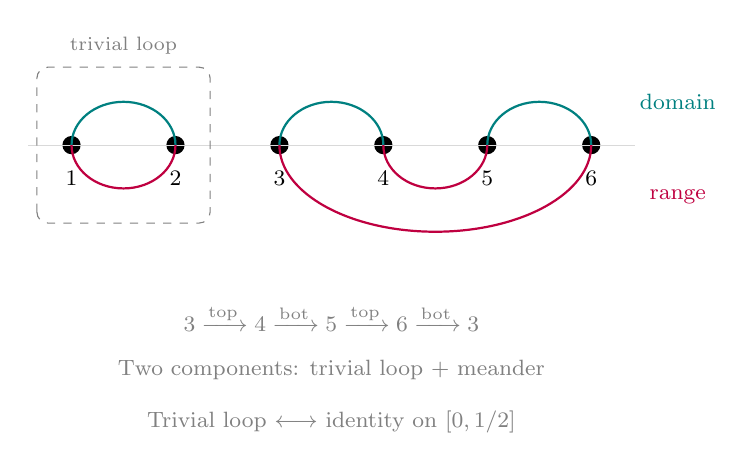
\begin{tikzpicture}[scale=1.1]
  % Points
  \foreach \i/\x in {1/0, 2/1.2, 3/2.4, 4/3.6, 5/4.8, 6/6.0} {
    \fill (\x, 0) circle (3pt);
    \node[below=6pt, font=\footnotesize] at (\x, 0) {$\i$};
  }

  % Horizontal line
  \draw[gray!30] (-0.5, 0) -- (6.5, 0);

  % Top arcs (domain): {1,2}, {3,4}, {5,6}
  \draw[teal, thick] (0,0) arc[start angle=180, end angle=0, x radius=0.6, y radius=0.5];
  \draw[teal, thick] (2.4,0) arc[start angle=180, end angle=0, x radius=0.6, y radius=0.5];
  \draw[teal, thick] (4.8,0) arc[start angle=180, end angle=0, x radius=0.6, y radius=0.5];
  \node[teal, font=\footnotesize] at (7, 0.5) {domain};

  % Bottom arcs (range): {1,2}, {3,6}, {4,5}
  \draw[purple, thick] (0,0) arc[start angle=180, end angle=360, x radius=0.6, y radius=0.5];
  \draw[purple, thick] (2.4,0) arc[start angle=180, end angle=360, x radius=1.8, y radius=1.0];
  \draw[purple, thick] (3.6,0) arc[start angle=180, end angle=360, x radius=0.6, y radius=0.5];
  \node[purple, font=\footnotesize] at (7, -0.6) {range};

  % Component labels
  \draw[gray, dashed, thin, rounded corners] (-0.4, -0.9) rectangle (1.6, 0.9);
  \node[font=\scriptsize, gray] at (0.6, 1.15) {trivial loop};

  \node[font=\footnotesize, gray] at (3, -2) {$3 \xrightarrow{\text{top}} 4 \xrightarrow{\text{bot}} 5 \xrightarrow{\text{top}} 6 \xrightarrow{\text{bot}} 3$};
  \node[font=\footnotesize, gray] at (3, -2.6) {Two components: trivial loop $+$ meander};
  \node[font=\footnotesize, gray] at (3, -3.2) {Trivial loop $\longleftrightarrow$ identity on $[0, 1/2]$};
\end{tikzpicture}
\end{center}

The pair $\{1,2\}$ appears in both the top and bottom pairings, forming a small closed loop that does not interact with the remaining points.  This reflects the fact that $x_1$ is the identity on $[0, 1/2]$.  The remaining points $\{3, 4, 5, 6\}$ form a single meander, corresponding to the nontrivial part of $x_1$ on $[1/2, 1]$ --- which is a rescaled copy of $x_0$.

\end{document}
